%    inicio del documento
% ============================================================================
\documentclass[11pt]{report}


%    preambulo, configuracion y paginas iniciales
% ============================================================================
% --- preambulo --- {{{
\usepackage[spanish,es-lcroman,es-nodecimaldot]{babel}
\usepackage{amsmath}
\usepackage{amsfonts}
\usepackage{amssymb}
\usepackage{units}
\usepackage{xcolor}
\usepackage{hyperref}
\usepackage{fontspec}
\usepackage{subfiles}
\usepackage{graphicx}
\usepackage{booktabs}
\usepackage{multirow}
\usepackage{eso-pic}
\usepackage{setspace}
\usepackage{chngcntr}
\usepackage{fancyhdr}
\usepackage{titlesec}
\usepackage{titletoc}
\usepackage{enumitem}
\usepackage{blindtext}
\usepackage[intoc]{nomencl}
\usepackage[letterpaper,left=3cm,right=2cm,top=2cm,bottom=2cm]{geometry}
\usepackage[justification=justified,labelfont=bf,
            font=scriptsize,margin=1.5cm,labelsep=period]{caption}
\usepackage[sort&compress,authoryear]{natbib}
%
% --- }}}

%  --- configuracion general --- {{{

% configuracion de la fuente
\DeclareTextFontCommand{\emph}{\slshape}
\renewcommand\familydefault{\sfdefault}

% marcados de los items en las listas
\renewcommand{\labelitemi}{$\bullet$}

% espaciado de las lineas para las págines iniciales
\renewcommand{\baselinestretch}{1} 

%  color de los links
\hypersetup{
    colorlinks,
        linkcolor={black},
        citecolor={blue!50!black},
        urlcolor={blue!80!black}
        }

% poner numero de pagina en la parte superior derecha
\pagestyle{fancy}
\fancyhf{}
%\rhead{\thepage}
\fancyhead[LE,RO]{\thepage}
\renewcommand{\headrulewidth}{0pt}
\makeatletter
\renewcommand\chapter{\if@openright\cleardoublepage\else\clearpage\fi
             \thispagestyle{fancy}%
             \global\@topnum\z@
             \@afterindentfalse
             \secdef\@chapter\@schapter}
\makeatother

% definicion de encabezados para paginas especiales
\fancypagestyle{special}
{
  \fancyhf{}
  \renewcommand\headrulewidth{0pt}
  \renewcommand\footrulewidth{0pt}
  \rhead{\thepage}
}
% --- }}}

%  --- definicion de variables --- {{{
\def\thesisyear{2018}
\def\thesisauthor{Daniel Santiago Peláez Zapata}
\def\thesistitle{Efecto del oleaje en la capa límite superficial del océano}
\def\thesissubject{Oceanografía Física}
\def\thesiskind{M.Sc.}
\def\thesiskindtitle{Maestro en Ciencias}
\def\thesiskindformal{Maestría en Ciencias}
\def\thesiscity{Ensenada}
\def\thesisstate{Baja California}
\def\thesiscountry{México}
\def\thesisuniversity{Centro de Investigación Científica y de Educación
                      Superior de Ensenada, Baja California}
\def\thesisschool{Departamento de Oceanografía Física}
\def\thesisgroup{Grupo de oleaje}
\def\thesiskeywords{oleaje, capa límite superficial, tasa de disipación de TKE,
                    interacción océano-atmósfera}
%
\def\thesistitleenglish{Effect of waves in the upper ocean boundary layer}
\def\thesissubjectenglish{Physical Oceanography}
\def\thesiskindtitleenglish{Master of Sciences}
\def\thesiskeywordsenglish{surface waves, surface boundary layer, dissipation
                          rate of TKE, air-sea interaction}
% --- }}}

%  --- definicion de funciones y macros --- {{{

%  crear todo-notes
\newcommand\todo[1]{\textcolor{blue!80!red}{\textbf{TODO:} #1}}

% function para escribir rapidamente nombre y cargo
\newcommand{\comite}[2]{#1 \\ {\small #2}}

% comando que pone las unidades a los numeros en modo texto
\newcommand{\num}[2]{\ensuremath{#1\,\mathrm{#2}}\!\,} %para que no joda el fold

% alias a la palabra Figura y Tabla
\newcommand{\fig}[0]{Fig.}
\newcommand{\tab}[0]{Tab.}

% otras
\newcommand{\swell}[0]{\emph{swell}}
% --- }}}

%  --- paginas iniciales --- {{{
\begin{document}

\begin{titlepage}

  %  primera pagina: portada --- {{{
  \newpage
  \thispagestyle{empty}
  %
  \begin{center}
    %
    \huge{\textbf{\thesisuniversity}} \\
    \vspace{1.9cm} 
    
\includegraphics[width=7cm]{frontmatter/logo_cicese.pdf} \\
    \vspace{0.9cm}
    %
    \vrule width 15.5cm height .5pt \\
    \huge{\textbf{\thesiskindformal~en \thesissubject}} \\
    \vrule width 15.5cm height .1pt \\
    \vspace{0.9cm}
    %
    \parbox{10cm}{
      \centering
      \LARGE{\textbf{\thesistitle}}
    } \\
    \vspace{1.9cm}
    %
    \normalsize{
      Tesis \\
      para cubrir parcialmente los requisitos necesarios para obtener el grado de \\ 
      \thesiskindtitle
    }
    \\
    \vspace{0.9cm}
    \large{Presenta:} \\
    \vspace{0.7cm}
    \textbf{\Large{\thesisauthor}} \\
    %
    \vfill
    \large{
      \thesiscity, \thesisstate, \thesiscountry \\
      \thesisyear
    }
    %
    \newpage
  \end{center}
  % --- }}}

  % segunda pagina: hoja de firmas --- {{{
  \newpage
  \thispagestyle{empty}
  \begin{center}
    Tesis defendida por:

    \Large{\bfseries{\thesisauthor}}
    \vspace{0.5cm}

    \normalsize{y aprobada por el siguiente Comité}
    \vspace{1.5cm}

    \rule{0.5\textwidth}{.5pt} \\
    \comite{Dr. Francisco Javier Ocampo Torres}{Director de tesis} \\
    \vfill
    Dr. Oscar Sosa Nishizaki    \\ \vspace{1em}
    Dr. José Pedro Osuna Cañedo \\ \vspace{1em}
    Dr. Héctor García Nava      \\ \vspace{1em}
    \vfill
    
\includegraphics[width=1.5cm]{frontmatter/oceanografia.jpg} \\
    \vfill
    \rule{0.5\textwidth}{.5pt} \\
    \comite{Dr. Cuauhtémoc Turrent Thompson}{Coordinador del Posgrado en
    Oceanografía Física} \\ \vspace{1em}
    \vfill
    \rule{0.5\textwidth}{.5pt} \\
    \comite{Dra. Rufina Hernández Martínez}{Directora de Estudios de Posgrado} \\
    \vfill
    \scriptsize{
      \textit{ \thesisauthor~\textcopyright~\thesisyear} \\ \vspace{1em}
      \textit{Queda prohibida la reproducción parcial o total de esta
      obra sin el permiso formal y explícito del autor y del director de tesis}
    }
  \end{center}
  % --- }}}

\end{titlepage}
% --- }}}

% --- configuracion del cuerpo --- {{{

% definir espaciado de parrafos
\setlength{\parindent}{0mm}

% establecer nuevo numero de pagina despues de iniciales
\pagenumbering{roman}
\setcounter{page}{2}

% cambiar titulos de secciones y captions
\renewcommand{\contentsname}{Tabla de contenido}
\renewcommand{\listfigurename}{Lista de figuras}
\renewcommand{\listtablename}{Lista de tablas}
\renewcommand{\appendixname}{Anexo}
\renewcommand{\bibname}{Literatura citada}
\renewcommand{\figurename}{Figura}
\renewcommand{\tablename}{Tabla}

% numeracion continua en ecuaciones, figuras y tablas
\counterwithout{equation}{chapter}
\counterwithout{figure}{chapter}
\counterwithout{table}{chapter}

% agregar palabra pagina en toc, lof y lot
\addtocontents{toc}{~\hfill\textbf{Página}\par}
\addtocontents{lof}{\textbf{Figura}~\hfill\textbf{Página}\par}
\addtocontents{lot}{\textbf{Tabla}~\hfill\textbf{Página}\par}

% agregar palabra capitulo en la toc
\titlecontents{chapter}% <section-type>
  [0pt]% <left>
  {\bfseries}% <above-code>
  {\chaptername\ \thecontentslabel.\quad}% <numbered-entry-format>
  {}% <numbered-entry-format>
  {\hfill\contentspage}% <filler-page-format>


% --- }}}

%  --- resumen en espanol --- {{{
\thispagestyle{special}
\addcontentsline{toc}{chapter}{Resumen en español}

Resumen de la tesis que presenta \thesisauthor~como requisito parcial para la
obtención del grado de \thesiskindtitle~en \thesissubject. 

\vspace{2em}
\begin{center}
  \Large{\textbf{\thesistitle}} \\
\end{center}

\vspace{1em}
Resumen aprobado por:
\vspace{1em}

\hfill
\parbox{0.5\textwidth}{
  \begin{center}
      \rule{0.5\textwidth}{.5pt} \\
      \comite{Dr. Francisco Javier Ocampo Torres}{Director de tesis}
  \end{center}
}

\vspace{3em}
\subfile{resumen.tex}
\vfill
\textbf{Palabras clave:} \thesiskeywords
% --- }}}

%  --- resumen en ingles --- {{{
\newpage
\thispagestyle{special}
\addcontentsline{toc}{chapter}{Resumen en inglés}

Abstract of the thesis presented by \thesisauthor~as a partial requirement to
obtain the \thesiskindtitleenglish~degree in \thesissubjectenglish. 

\vspace{2em}
\begin{center}
  \Large{\textbf{\thesistitleenglish}} \\
\end{center}

\vspace{1em}
Abstract approved by:
\vspace{1em}

\hfill
\parbox{0.5\textwidth}{
  \begin{center}
      \rule{0.5\textwidth}{.5pt} \\
      \comite{Dr. Francisco Javier Ocampo Torres}{Thesis Advisor}
  \end{center}
}

\vspace{3em}
\subfile{abstract.tex}
\vfill
\textbf{Palabras clave:} \thesiskeywordsenglish
% --- }}}

% --- dedicatoria --- {{{
\newcommand\backgroundpic{
  \put(0,0){
    \parbox[b][\paperheight]{\paperwidth}{
      \vfill
      \centering
      \hspace*{-0.6cm}
      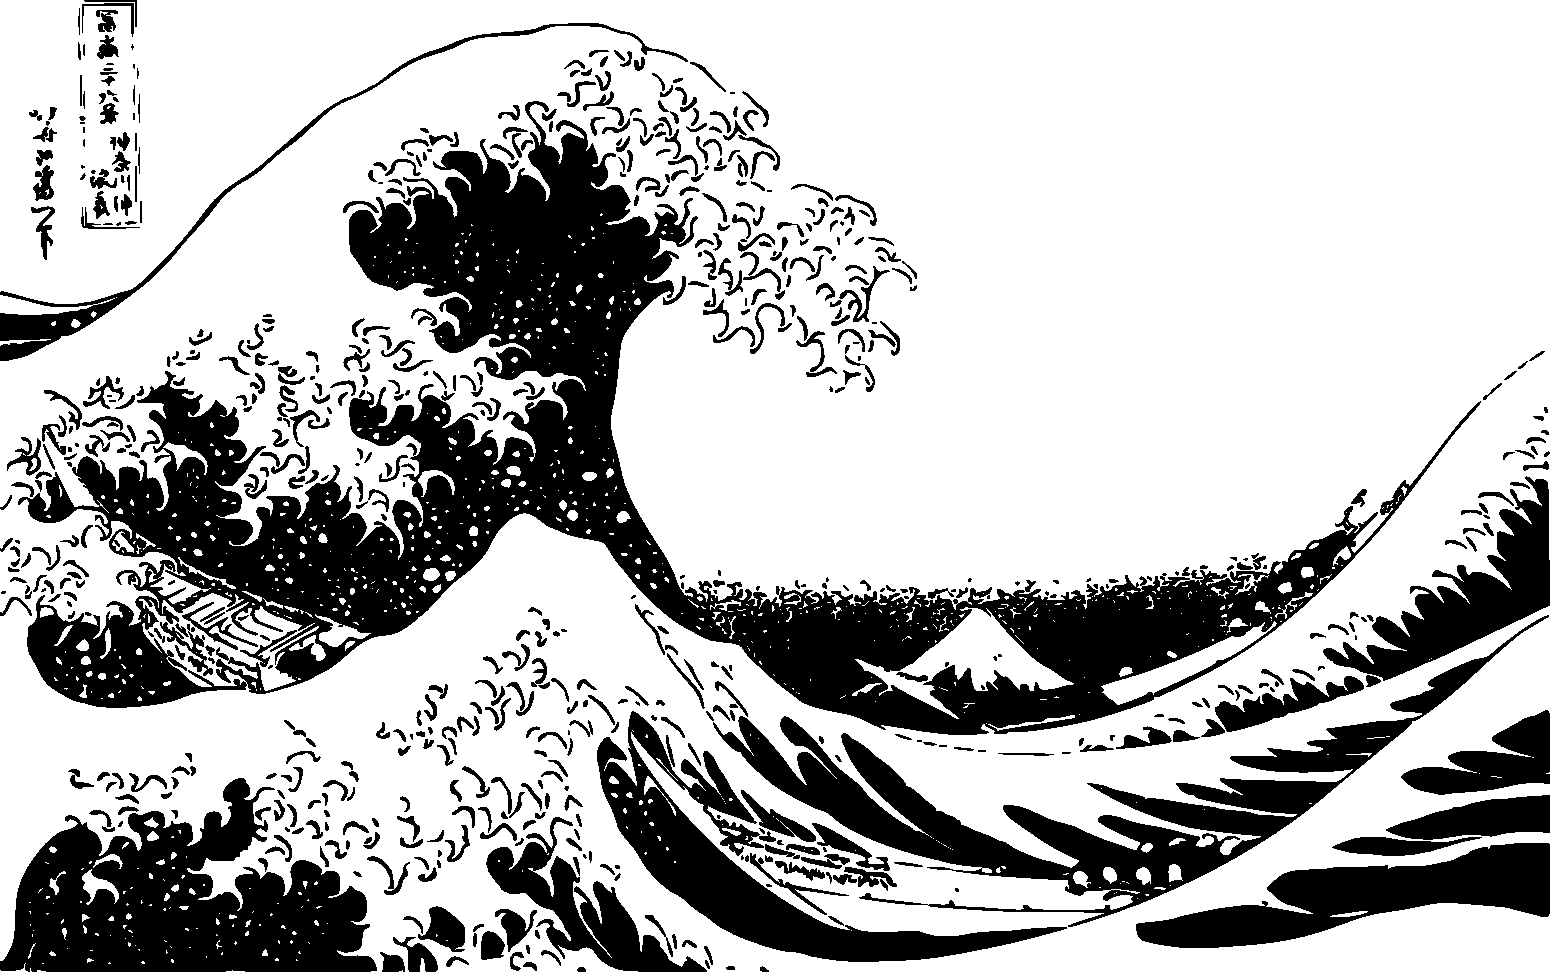
\includegraphics[width=\paperwidth,height=0.35\paperheight]{frontmatter/background.pdf}
    }
  }
}
\setlength{\parindent}{0cm}
\newpage
\thispagestyle{empty}
\begin{flushright}
  \vspace*{5cm}
  %
  \emph{"<Big whirls have little whirls that feed on their velocity, \\
        and little whirls have lesser whirls and so on to viscosity.">}\\
  %
  \vspace*{1em}
  \footnotesize{L. F. Richardson}
  %
  \AddToShipoutPicture*{\backgroundpic}
  \vfill
\end{flushright}
% --- }}}

%  --- pagina de agradecimientos --- {{{

% un espacio y medio para el cuerpo del documento
\doublespacing

% preconfiguracion de las secciones para los argradecimientos y las tablas
\titleformat{\chapter}[hang]{\centering\normalfont\LARGE\bfseries}{}{0pt}{\LARGE}
\titlespacing*{\chapter}{0pt}{-16pt}{16pt}

\chapter*{Agradecimientos}
\addcontentsline{toc}{chapter}{Agradecimientos}
\subfile{acknowledgments.tex}
% --- }}}

%  --- tablas de contenido --- {{{
\renewcommand{\contentsname}{\bfseries\LARGE Tabla de contenido}
\renewcommand{\listfigurename}{\bfseries\LARGE Lista de figuras}
\renewcommand{\listtablename}{\bfseries\LARGE Lista de tablas}
%
\newpage
\tableofcontents
%
\newpage
\addcontentsline{toc}{chapter}{Lista de figuras}
\listoffigures
%
\newpage
\addcontentsline{toc}{chapter}{Lista de tablas}
\listoftables
% --- }}}

% --- re-configuracion del formato de las secciones --- {{{
%
% restaurar numberos arabigos
\clearpage
\pagenumbering{arabic}
\setcounter{page}{1}

% formato del titulo
\titleformat{\chapter}[hang]
  {\normalfont\LARGE\bfseries}
  {\chaptertitlename\ \thechapter.}
  {16pt}
  {\LARGE}
  [\vspace{1ex}\titlerule]
\titlespacing*{\chapter}{0pt}{-16pt}{16pt}

% espaciado de titulos de secciones (recomendacion de cicese)
%\titlespacing\chapter{0pt}{-40.25pt plus 4pt minus 2pt}{12pt plus 2pt minus 2pt}
%\titlespacing\section{0pt}{0pt plus 4pt minus 2pt}{3pt plus 2pt minus 2pt}
%\titlespacing\subsection{0pt}{0pt plus 4pt minus 2pt}{3pt plus 2pt minus 2pt}
%\titlespacing\subsubsection{0pt}{0pt plus 4pt minus 2pt}{3pt plus 2pt minus 2pt}

% espaciado entre parragos (recomendacion de cicese)
\setlength{\parskip}{12pt plus 1pt minus 1pt}

% --- }}}


%    cuerpo del documento
% ============================================================================
%  --- incluir capitulos --- {{{
\subfile{chapter01}
\subfile{chapter02}
\subfile{chapter03}
\subfile{chapter04}
% --- }}}

%  --- incluir referencias --- {{{
\newpage
\singlespacing
\addcontentsline{toc}{chapter}{Literatura citada}
\bibliographystyle{cicese}
\bibliography{./references.bib}
% --- }}}

%  --- incluir apendices --- {{{
% \appendix
% \subfile{appendix01}
% --- }}}


%    terminar documento
% ============================================================================
\end{document}
